% Options for packages loaded elsewhere
\PassOptionsToPackage{unicode}{hyperref}
\PassOptionsToPackage{hyphens}{url}
%
\documentclass[
]{book}
\usepackage{amsmath,amssymb}
\usepackage{lmodern}
\usepackage{ifxetex,ifluatex}
\ifnum 0\ifxetex 1\fi\ifluatex 1\fi=0 % if pdftex
  \usepackage[T1]{fontenc}
  \usepackage[utf8]{inputenc}
  \usepackage{textcomp} % provide euro and other symbols
\else % if luatex or xetex
  \usepackage{unicode-math}
  \defaultfontfeatures{Scale=MatchLowercase}
  \defaultfontfeatures[\rmfamily]{Ligatures=TeX,Scale=1}
\fi
% Use upquote if available, for straight quotes in verbatim environments
\IfFileExists{upquote.sty}{\usepackage{upquote}}{}
\IfFileExists{microtype.sty}{% use microtype if available
  \usepackage[]{microtype}
  \UseMicrotypeSet[protrusion]{basicmath} % disable protrusion for tt fonts
}{}
\makeatletter
\@ifundefined{KOMAClassName}{% if non-KOMA class
  \IfFileExists{parskip.sty}{%
    \usepackage{parskip}
  }{% else
    \setlength{\parindent}{0pt}
    \setlength{\parskip}{6pt plus 2pt minus 1pt}}
}{% if KOMA class
  \KOMAoptions{parskip=half}}
\makeatother
\usepackage{xcolor}
\IfFileExists{xurl.sty}{\usepackage{xurl}}{} % add URL line breaks if available
\IfFileExists{bookmark.sty}{\usepackage{bookmark}}{\usepackage{hyperref}}
\hypersetup{
  pdftitle={A GitBook template},
  pdfauthor={Nikola Sekulovski},
  hidelinks,
  pdfcreator={LaTeX via pandoc}}
\urlstyle{same} % disable monospaced font for URLs
\usepackage{color}
\usepackage{fancyvrb}
\newcommand{\VerbBar}{|}
\newcommand{\VERB}{\Verb[commandchars=\\\{\}]}
\DefineVerbatimEnvironment{Highlighting}{Verbatim}{commandchars=\\\{\}}
% Add ',fontsize=\small' for more characters per line
\usepackage{framed}
\definecolor{shadecolor}{RGB}{248,248,248}
\newenvironment{Shaded}{\begin{snugshade}}{\end{snugshade}}
\newcommand{\AlertTok}[1]{\textcolor[rgb]{0.94,0.16,0.16}{#1}}
\newcommand{\AnnotationTok}[1]{\textcolor[rgb]{0.56,0.35,0.01}{\textbf{\textit{#1}}}}
\newcommand{\AttributeTok}[1]{\textcolor[rgb]{0.77,0.63,0.00}{#1}}
\newcommand{\BaseNTok}[1]{\textcolor[rgb]{0.00,0.00,0.81}{#1}}
\newcommand{\BuiltInTok}[1]{#1}
\newcommand{\CharTok}[1]{\textcolor[rgb]{0.31,0.60,0.02}{#1}}
\newcommand{\CommentTok}[1]{\textcolor[rgb]{0.56,0.35,0.01}{\textit{#1}}}
\newcommand{\CommentVarTok}[1]{\textcolor[rgb]{0.56,0.35,0.01}{\textbf{\textit{#1}}}}
\newcommand{\ConstantTok}[1]{\textcolor[rgb]{0.00,0.00,0.00}{#1}}
\newcommand{\ControlFlowTok}[1]{\textcolor[rgb]{0.13,0.29,0.53}{\textbf{#1}}}
\newcommand{\DataTypeTok}[1]{\textcolor[rgb]{0.13,0.29,0.53}{#1}}
\newcommand{\DecValTok}[1]{\textcolor[rgb]{0.00,0.00,0.81}{#1}}
\newcommand{\DocumentationTok}[1]{\textcolor[rgb]{0.56,0.35,0.01}{\textbf{\textit{#1}}}}
\newcommand{\ErrorTok}[1]{\textcolor[rgb]{0.64,0.00,0.00}{\textbf{#1}}}
\newcommand{\ExtensionTok}[1]{#1}
\newcommand{\FloatTok}[1]{\textcolor[rgb]{0.00,0.00,0.81}{#1}}
\newcommand{\FunctionTok}[1]{\textcolor[rgb]{0.00,0.00,0.00}{#1}}
\newcommand{\ImportTok}[1]{#1}
\newcommand{\InformationTok}[1]{\textcolor[rgb]{0.56,0.35,0.01}{\textbf{\textit{#1}}}}
\newcommand{\KeywordTok}[1]{\textcolor[rgb]{0.13,0.29,0.53}{\textbf{#1}}}
\newcommand{\NormalTok}[1]{#1}
\newcommand{\OperatorTok}[1]{\textcolor[rgb]{0.81,0.36,0.00}{\textbf{#1}}}
\newcommand{\OtherTok}[1]{\textcolor[rgb]{0.56,0.35,0.01}{#1}}
\newcommand{\PreprocessorTok}[1]{\textcolor[rgb]{0.56,0.35,0.01}{\textit{#1}}}
\newcommand{\RegionMarkerTok}[1]{#1}
\newcommand{\SpecialCharTok}[1]{\textcolor[rgb]{0.00,0.00,0.00}{#1}}
\newcommand{\SpecialStringTok}[1]{\textcolor[rgb]{0.31,0.60,0.02}{#1}}
\newcommand{\StringTok}[1]{\textcolor[rgb]{0.31,0.60,0.02}{#1}}
\newcommand{\VariableTok}[1]{\textcolor[rgb]{0.00,0.00,0.00}{#1}}
\newcommand{\VerbatimStringTok}[1]{\textcolor[rgb]{0.31,0.60,0.02}{#1}}
\newcommand{\WarningTok}[1]{\textcolor[rgb]{0.56,0.35,0.01}{\textbf{\textit{#1}}}}
\usepackage{longtable,booktabs,array}
\usepackage{calc} % for calculating minipage widths
% Correct order of tables after \paragraph or \subparagraph
\usepackage{etoolbox}
\makeatletter
\patchcmd\longtable{\par}{\if@noskipsec\mbox{}\fi\par}{}{}
\makeatother
% Allow footnotes in longtable head/foot
\IfFileExists{footnotehyper.sty}{\usepackage{footnotehyper}}{\usepackage{footnote}}
\makesavenoteenv{longtable}
\usepackage{graphicx}
\makeatletter
\def\maxwidth{\ifdim\Gin@nat@width>\linewidth\linewidth\else\Gin@nat@width\fi}
\def\maxheight{\ifdim\Gin@nat@height>\textheight\textheight\else\Gin@nat@height\fi}
\makeatother
% Scale images if necessary, so that they will not overflow the page
% margins by default, and it is still possible to overwrite the defaults
% using explicit options in \includegraphics[width, height, ...]{}
\setkeys{Gin}{width=\maxwidth,height=\maxheight,keepaspectratio}
% Set default figure placement to htbp
\makeatletter
\def\fps@figure{htbp}
\makeatother
\setlength{\emergencystretch}{3em} % prevent overfull lines
\providecommand{\tightlist}{%
  \setlength{\itemsep}{0pt}\setlength{\parskip}{0pt}}
\setcounter{secnumdepth}{5}
\usepackage{booktabs}
\usepackage{amsthm}
\makeatletter
\def\thm@space@setup{%
  \thm@preskip=8pt plus 2pt minus 4pt
  \thm@postskip=\thm@preskip
}
\makeatother
\usepackage{booktabs}
\usepackage{longtable}
\usepackage{array}
\usepackage{multirow}
\usepackage{wrapfig}
\usepackage{float}
\usepackage{colortbl}
\usepackage{pdflscape}
\usepackage{tabu}
\usepackage{threeparttable}
\usepackage{threeparttablex}
\usepackage[normalem]{ulem}
\usepackage{makecell}
\usepackage{xcolor}
\ifluatex
  \usepackage{selnolig}  % disable illegal ligatures
\fi
\newlength{\cslhangindent}
\setlength{\cslhangindent}{1.5em}
\newlength{\csllabelwidth}
\setlength{\csllabelwidth}{3em}
\newenvironment{CSLReferences}[2] % #1 hanging-ident, #2 entry spacing
 {% don't indent paragraphs
  \setlength{\parindent}{0pt}
  % turn on hanging indent if param 1 is 1
  \ifodd #1 \everypar{\setlength{\hangindent}{\cslhangindent}}\ignorespaces\fi
  % set entry spacing
  \ifnum #2 > 0
  \setlength{\parskip}{#2\baselineskip}
  \fi
 }%
 {}
\usepackage{calc}
\newcommand{\CSLBlock}[1]{#1\hfill\break}
\newcommand{\CSLLeftMargin}[1]{\parbox[t]{\csllabelwidth}{#1}}
\newcommand{\CSLRightInline}[1]{\parbox[t]{\linewidth - \csllabelwidth}{#1}\break}
\newcommand{\CSLIndent}[1]{\hspace{\cslhangindent}#1}

\title{A GitBook template}
\author{Nikola Sekulovski}
\date{2021-10-27}

\begin{document}
\maketitle

{
\setcounter{tocdepth}{1}
\tableofcontents
}
\hypertarget{introduction}{%
\chapter{Introduction}\label{introduction}}

This is a template GitBook based on \href{https://cjvanlissa.github.io/gitbook-demo/}{\emph{A GitBook Example for Teaching}} and \href{https://bookdown.org/yihui/bookdown/}{\emph{bookdown: Authoring Books and Technical Documents with R Markdown}}.

This is how we would reference a book (\protect\hyperlink{ref-xie2015}{Xie, 2015}) or \protect\hyperlink{ref-xie2015}{Xie} (\protect\hyperlink{ref-xie2015}{2015}).

This is how we would reference articles \protect\hyperlink{ref-gu2018approximated}{Gu, Mulder, \& Hoijtink} (\protect\hyperlink{ref-gu2018approximated}{2018}) or (\protect\hyperlink{ref-hoijtink2008bayesian}{Hoijtink, Klugkist, \& Boelen, 2008}).

\hypertarget{monte-carlo-simulations}{%
\chapter{Monte Carlo Simulations}\label{monte-carlo-simulations}}

\begin{Shaded}
\begin{Highlighting}[]
\FunctionTok{library}\NormalTok{(tidyverse)}
\end{Highlighting}
\end{Shaded}

\hypertarget{the-confidence-interval}{%
\section{The Confidence Interval}\label{the-confidence-interval}}

In this exercise I will try to repeat the example given by \href{https://www.gerkovink.com/markup/Wk1/Solution_to_Ex1.html}{Gerko Vink}

The main idea of this exercise is to illustrate the nature of the \emph{Confidence Interval} as described by \href{http://www.stat.cmu.edu/~brian/905-2008/papers/neyman-1934-jrss.pdf}{Neyman (1934)}

We set a seed to make our results reproducible:

\begin{Shaded}
\begin{Highlighting}[]
\FunctionTok{set.seed}\NormalTok{(}\DecValTok{6465}\NormalTok{)}
\end{Highlighting}
\end{Shaded}

\begin{itemize}
\tightlist
\item
  The first step is to take 100 samples (in this case of size 800) from a \emph{normal distributuon} with \(\mu = 0\) and \(\sigma = 1\):
\end{itemize}

\begin{Shaded}
\begin{Highlighting}[]
\NormalTok{samples }\OtherTok{\textless{}{-}}\NormalTok{plyr}\SpecialCharTok{::}\FunctionTok{rlply}\NormalTok{(}\DecValTok{100}\NormalTok{, }\FunctionTok{rnorm}\NormalTok{(}\DecValTok{800}\NormalTok{, }\DecValTok{0}\NormalTok{, }\DecValTok{1}\NormalTok{))}
\end{Highlighting}
\end{Shaded}

\begin{itemize}
\tightlist
\item
  Secondly, we need to calculate for the mean of each sample: the absolute bias; standard error lower bound of the 95\% confidence interval and upper bound of the 95\% confidence interval.
\end{itemize}

We can construct a function that does this:

\begin{Shaded}
\begin{Highlighting}[]
\NormalTok{samp\_function }\OtherTok{\textless{}{-}} \ControlFlowTok{function}\NormalTok{(x) \{}
 
\NormalTok{  m }\OtherTok{\textless{}{-}} \FunctionTok{mean}\NormalTok{(x)}
\NormalTok{  n }\OtherTok{\textless{}{-}} \FunctionTok{length}\NormalTok{(x)}
\NormalTok{  se }\OtherTok{\textless{}{-}} \DecValTok{1}\SpecialCharTok{/}\FunctionTok{sqrt}\NormalTok{(n)}
\NormalTok{  bias }\OtherTok{\textless{}{-}} \FunctionTok{abs}\NormalTok{(}\SpecialCharTok{{-}}\DecValTok{0} \SpecialCharTok{{-}}\NormalTok{ m)}
\NormalTok{  df }\OtherTok{\textless{}{-}}\NormalTok{ n }\SpecialCharTok{{-}} \DecValTok{1}
\NormalTok{  interval }\OtherTok{\textless{}{-}} \FunctionTok{qt}\NormalTok{(.}\DecValTok{975}\NormalTok{, df) }\SpecialCharTok{*}\NormalTok{ se}
  \FunctionTok{return}\NormalTok{(}\FunctionTok{c}\NormalTok{(m, bias, se, m }\SpecialCharTok{{-}}\NormalTok{ interval, m }\SpecialCharTok{+}\NormalTok{ interval))}

\NormalTok{\}}

\NormalTok{format }\OtherTok{\textless{}{-}} \FunctionTok{c}\NormalTok{(}\StringTok{"Mean"} \OtherTok{=} \DecValTok{0}\NormalTok{, }\StringTok{"Bias"} \OtherTok{=} \DecValTok{0}\NormalTok{, }\StringTok{"Std.Err"} \OtherTok{=} \DecValTok{0}\NormalTok{, }\StringTok{"Lower"} \OtherTok{=} \DecValTok{0}\NormalTok{, }\StringTok{"Upper"} \OtherTok{=} \DecValTok{0}\NormalTok{)}
\end{Highlighting}
\end{Shaded}

Now we use the constructed function \texttt{samp\_function} on all 100 samples contained in the object \texttt{samples}. And we also add a new column to the results that indicates which CI of the respective samples does contain \(\mu\).

\begin{Shaded}
\begin{Highlighting}[]
\NormalTok{results }\OtherTok{\textless{}{-}}\NormalTok{ samples }\SpecialCharTok{\%\textgreater{}\%}
  \FunctionTok{vapply}\NormalTok{(., samp\_function, format) }\SpecialCharTok{\%\textgreater{}\%}
\NormalTok{  t }\SpecialCharTok{\%\textgreater{}\%}
\NormalTok{  as\_tibble }\SpecialCharTok{\%\textgreater{}\%} 
  \FunctionTok{mutate}\NormalTok{(}\AttributeTok{Covered =} \FunctionTok{ifelse}\NormalTok{(Lower }\SpecialCharTok{\textless{}} \DecValTok{0} \SpecialCharTok{\&}\NormalTok{ Upper }\SpecialCharTok{\textgreater{}} \DecValTok{0}\NormalTok{, }\DecValTok{1}\NormalTok{, }\DecValTok{0}\NormalTok{))}
\end{Highlighting}
\end{Shaded}

We can also add a table with the sample statistics of the samples whose CI's do not contain \(\mu\).

\begin{Shaded}
\begin{Highlighting}[]
\NormalTok{results }\SpecialCharTok{\%\textgreater{}\%}
  \FunctionTok{filter}\NormalTok{(Covered }\SpecialCharTok{==}\DecValTok{0}\NormalTok{) }\SpecialCharTok{\%\textgreater{}\%}
\NormalTok{  kableExtra}\SpecialCharTok{::}\FunctionTok{kable}\NormalTok{(}\AttributeTok{caption =} \StringTok{"Here is a table of the samples"}\NormalTok{ )}
\end{Highlighting}
\end{Shaded}

\begin{table}

\caption{\label{tab:unnamed-chunk-6}Here is a table of the samples}
\centering
\begin{tabular}[t]{r|r|r|r|r|r}
\hline
Mean & Bias & Std.Err & Lower & Upper & Covered\\
\hline
-0.0945589 & 0.0945589 & 0.0353553 & -0.1639592 & -0.0251585 & 0\\
\hline
0.0740058 & 0.0740058 & 0.0353553 & 0.0046055 & 0.1434062 & 0\\
\hline
\end{tabular}
\end{table}

And finally we can also make a nice plot illustrating everything that we did so far.

\begin{Shaded}
\begin{Highlighting}[]
\NormalTok{lims }\OtherTok{\textless{}{-}} \FunctionTok{aes}\NormalTok{(}\AttributeTok{ymax =}\NormalTok{ results}\SpecialCharTok{$}\NormalTok{Upper, }\AttributeTok{ymin =}\NormalTok{ results}\SpecialCharTok{$}\NormalTok{Lower)}
\FunctionTok{ggplot}\NormalTok{(results, }\FunctionTok{aes}\NormalTok{(}\AttributeTok{y=}\NormalTok{Mean, }\AttributeTok{x=}\DecValTok{1}\SpecialCharTok{:}\DecValTok{100}\NormalTok{, }\AttributeTok{colour =}\NormalTok{ Covered)) }\SpecialCharTok{+} 
  \FunctionTok{geom\_hline}\NormalTok{(}\FunctionTok{aes}\NormalTok{(}\AttributeTok{yintercept =} \DecValTok{0}\NormalTok{)) }\SpecialCharTok{+} 
  \FunctionTok{geom\_pointrange}\NormalTok{(lims) }\SpecialCharTok{+} 
  \FunctionTok{xlab}\NormalTok{(}\StringTok{"Simulations"}\NormalTok{) }\SpecialCharTok{+}
  \FunctionTok{ylab}\NormalTok{(}\StringTok{"Means and 95\% Confidence Intervals"}\NormalTok{)}
\end{Highlighting}
\end{Shaded}

\begin{verbatim}
## Warning: Use of `results$Upper` is discouraged. Use `Upper` instead.
\end{verbatim}

\begin{verbatim}
## Warning: Use of `results$Lower` is discouraged. Use `Lower` instead.
\end{verbatim}

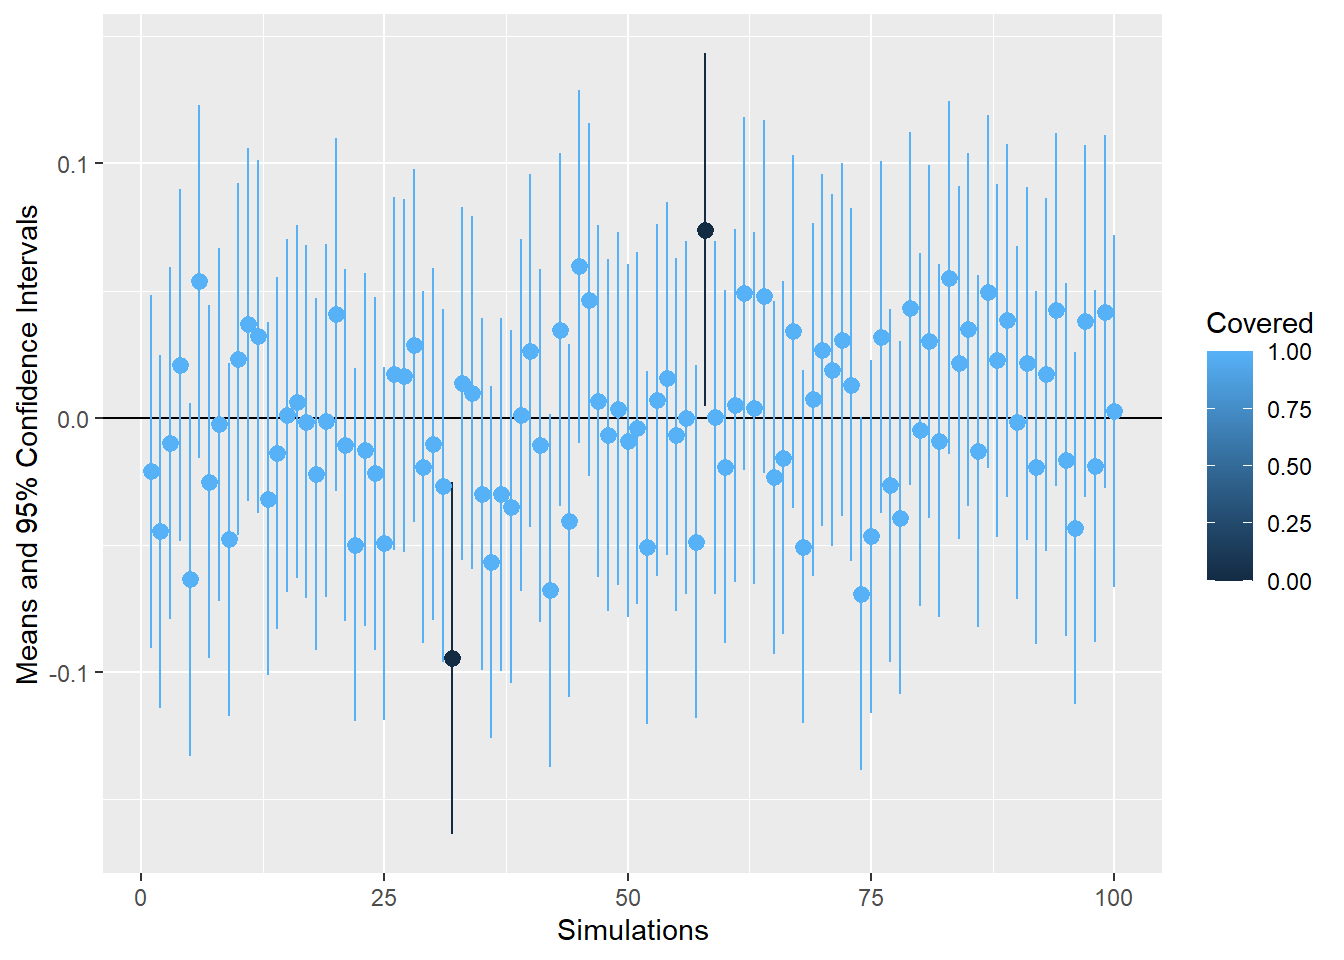
\includegraphics{gitbook-template-_files/figure-latex/unnamed-chunk-7-1.pdf}
In this case only two out of 100 CI's do not include the true population mean.

\hypertarget{the-central-limit-theorem}{%
\section{The Central Limit Theorem}\label{the-central-limit-theorem}}

Here we will also try to illustrate the \href{https://en.wikipedia.org/wiki/Central_limit_theorem}{Central Limit Theorem}, in it's most basic form, with a very simple example.

First we draw 1000 samples (again of size 800), form , say, a \emph{Poisson} distribution, of course we could've drawn them from a uniform or an exponential as well.

\begin{Shaded}
\begin{Highlighting}[]
\NormalTok{samples\_2 }\OtherTok{\textless{}{-}}\NormalTok{ samples }\OtherTok{\textless{}{-}}\NormalTok{plyr}\SpecialCharTok{::}\FunctionTok{rlply}\NormalTok{(}\DecValTok{1000}\NormalTok{, }\FunctionTok{rpois}\NormalTok{(}\DecValTok{800}\NormalTok{, }\DecValTok{2}\NormalTok{))}
\end{Highlighting}
\end{Shaded}

Now we calculate the mean for each sample:

\begin{Shaded}
\begin{Highlighting}[]
\NormalTok{means }\OtherTok{\textless{}{-}}\NormalTok{ samples\_2 }\SpecialCharTok{\%\textgreater{}\%}
  \FunctionTok{lapply}\NormalTok{(., mean) }\SpecialCharTok{\%\textgreater{}\%}
  \FunctionTok{as.data.frame}\NormalTok{() }\SpecialCharTok{\%\textgreater{}\%}
  \FunctionTok{t}\NormalTok{()}
\end{Highlighting}
\end{Shaded}

And now we plot a histogram of the resulting means:

\begin{Shaded}
\begin{Highlighting}[]
\FunctionTok{hist}\NormalTok{(}\FunctionTok{t}\NormalTok{(means))}
\end{Highlighting}
\end{Shaded}

\begin{figure}
\centering
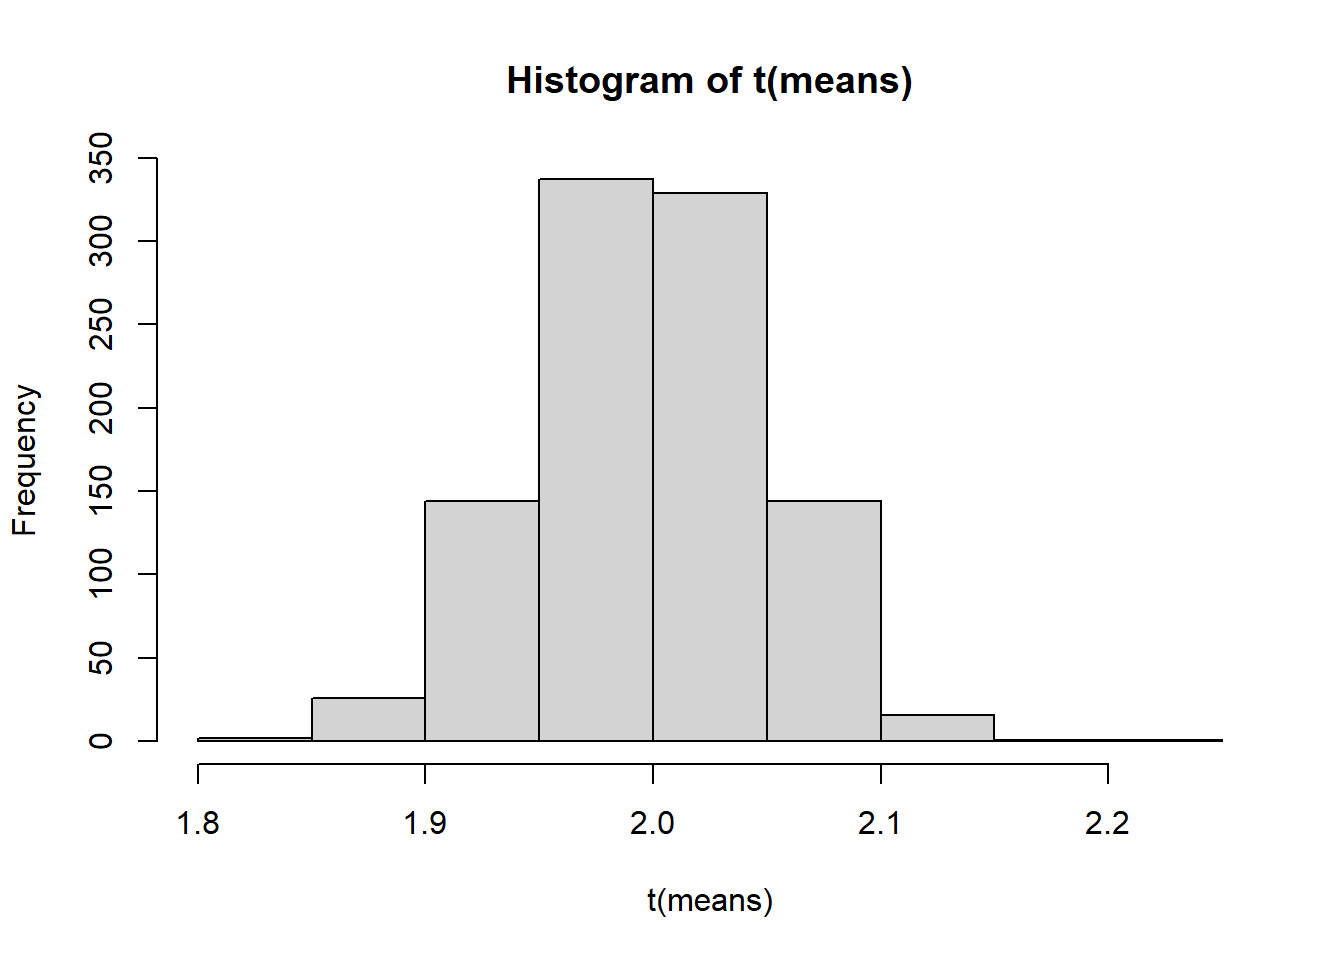
\includegraphics{gitbook-template-_files/figure-latex/unnamed-chunk-10-1.pdf}
\caption{\label{fig:unnamed-chunk-10}Histogram of the sampling distribution of the mean}
\end{figure}

\hypertarget{equations-picture}{%
\chapter{Equations \& Picture}\label{equations-picture}}

\hypertarget{bayes-theorem}{%
\section{Bayes' theorem}\label{bayes-theorem}}

\begin{equation} 
p(\theta | D) = \frac{p(D|\theta) p(\theta)} {p(D)}
\label{eq:bayes}
\end{equation}

\hypertarget{normal-pdf}{%
\section{Normal PDF}\label{normal-pdf}}

\begin{equation} 
f(x) = \frac{1}{\sigma\sqrt{2\pi}}\exp\left(-\frac{1}{2}\left(\frac{x-\mu}{\sigma}\right)^{2}\right)
\label{eq:normal}
\end{equation}

This is how we refer to equations:
-see equation \eqref{eq:normal}

\hypertarget{picture}{%
\section{Picture}\label{picture}}

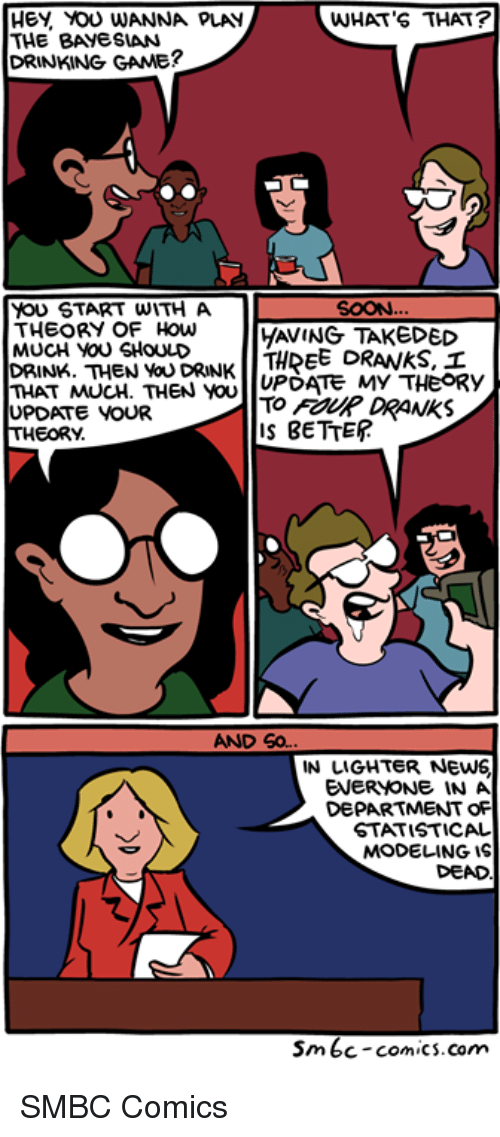
\includegraphics[width=6.94in]{images/Joke}

\hypertarget{part-r-package-bain}{%
\chapter*{\texorpdfstring{(PART) \texttt{R} package \texttt{bain}}{(PART) R package bain}}\label{part-r-package-bain}}
\addcontentsline{toc}{chapter}{(PART) \texttt{R} package \texttt{bain}}

\hypertarget{an-introduction-to-bain}{%
\chapter*{\texorpdfstring{An introduction to \texttt{bain}}{An introduction to bain}}\label{an-introduction-to-bain}}
\addcontentsline{toc}{chapter}{An introduction to \texttt{bain}}

\texttt{bain} is an acronym for ``Bayesian informative hypotheses evaluation.''
It uses the Bayes factor (\protect\hyperlink{ref-kass1995bayes}{Kass \& Raftery, 1995}) to evaluate hypotheses specified using \emph{equality} and \emph{inequality} constraints among (linear combinations of) parameters in a wide range of statistical models.

\hypertarget{available-tutorials}{%
\section{Available tutorials}\label{available-tutorials}}

Two tutorials are retrievable from the \texttt{bain} \href{https://informative-hypotheses.sites.uu.nl/software/bain/}{website} under the section \textbf{Tutorials}.

The first introducing Bayesian evaluation of informative hypotheses is provided by \protect\hyperlink{ref-e575e990fdef4c469a1c19a210d58e2f}{Hoijtink, Mulder, van Lissa, \& Gu} (\protect\hyperlink{ref-e575e990fdef4c469a1c19a210d58e2f}{2019}). By reading the tutorial in combination with executing the analyses contained in \texttt{easyBFtutorial.R} and \texttt{BFtutorial.R} (available on the abovementioned website) you will quickly learn the basics of Bayesian hypothesis evaluation.

The second containing introduction to Bayesian evaluation of informative hypotheses in the context of structural equation models is provided by Van Lissa, C., Gu, X., Mulder, J., Rosseel, Y., van Zundert, C. and Hoijtink, H. (2020), Structural Equation Modelling, 28, 292-301\footnote{Users are
  advised to read these tutorials and this vignette before using \texttt{bain}.}.

\textbf{Users are
advised to read these tutorials and this vignette before using \texttt{bain}}.

An overview of all other relevant papers concearning informative hypotheses testing and the package \texttt{bain} can be found \href{https://informative-hypotheses.sites.uu.nl/publications/}{here}.

\hypertarget{usage}{%
\section{Usage}\label{usage}}

This is how a general call to \texttt{bain} looks like:

\texttt{results\ \ \textless{}-\ bain(x,\ hypothesis,\ fraction\ =\ 1,\ ...)}

\hypertarget{arguments}{%
\subsection{Arguments}\label{arguments}}

\texttt{x}
An R object containing the outcome of a statistical analysis. Currently, the following objects can be processed:

\begin{enumerate}
\def\labelenumi{\arabic{enumi})}
\tightlist
\item
  \texttt{t\_test()} objects (Student's t-test, Welch's t-test, paired samples t-test, one-group t-test, equivalence test). Note that, \texttt{t\_test} can be used in the same way as \texttt{t.test}.
\item
  \texttt{lm()} objects (ANOVA, ANCOVA, multiple regression).
\item
  \texttt{lavaan} objects generated with the \texttt{sem()}, \texttt{cfa()}, and
  \texttt{growth} functions.
\item
  A named vector containing the estimates resulting from a statistical analysis. Using this option triggers the \texttt{bain.default()} method. Note that, named means that each estimate has to be named such that it can be referred to in hypotheses.
\item
  Wrapper functions for repeated measures ANOVA(\ldots) and linear two-level models built with \texttt{lmer} (TBA when finished)
\end{enumerate}

\texttt{hypothesis} A character string containing the informative hypotheses to evaluate
(see below the section on \textbf{``Specification of Hypotheses''}).

\texttt{fraction\ =\ 1} A number representing the fraction of information in the data used to construct the prior distribution (see, for example, \protect\hyperlink{ref-gu2018approximated}{Gu, Mulder, \& Hoijtink} (\protect\hyperlink{ref-gu2018approximated}{2018})). The default value 1 denotes the minimal fraction, 2 denotes twice the minimal fraction, etc. The examples in the next chapter show how the \texttt{fraction} can be employed to execute a sensitivity analysis. See also \protect\hyperlink{ref-e575e990fdef4c469a1c19a210d58e2f}{Hoijtink, Mulder, van Lissa, \& Gu} (\protect\hyperlink{ref-e575e990fdef4c469a1c19a210d58e2f}{2019}) for more details.

\texttt{...} Additional arguments (see next chapter).

\hypertarget{using-bain-with-a-lm-or-t_test-object}{%
\subsection{\texorpdfstring{Using \texttt{bain} with a \texttt{lm} or \texttt{t\_test} object}{Using bain with a lm or t\_test object}}\label{using-bain-with-a-lm-or-t_test-object}}

The following steps need to be executed:

\begin{enumerate}
\def\labelenumi{\arabic{enumi})}
\tightlist
\item
  \texttt{x\ \textless{}-\ lm()} or \texttt{x\ \textless{}-\ t\_test()}. Execute an analysis with
  \texttt{lm} or \texttt{t\_test}. See the Examples section below for a complete elaboration
  of the
  calls to \texttt{lm} and \texttt{t\_test} that can be processed by \texttt{bain}.
  Note that, \texttt{lm} and \texttt{t\_test} will apply list-wise deletion if there
  are cases with missing values in the variables used.
\item
  If \texttt{lm()} is used, display the estimates and their names using the command \texttt{coef(x)}. (Unique abbreviations of) the names will be used to specify \texttt{hypotheses}. If \texttt{t\_test()} is used, hypotheses have to be specified using the names \texttt{x}, \texttt{y}, and \texttt{difference} (see Examples 1a throught 1e which can be found below).
\item
  \texttt{set.seed(seed)}. Set \texttt{seed} equal to an integer
  number to create a repeatable random number sequence. \texttt{bain} uses sampling to compute Bayes factors and posterior model probabilities. It is therefore recommended to run analyses with two different seeds to ensure stability of the results.
\item
  \texttt{results\ \textless{}-\ bain(x,hypotheses,fraction\ =\ 1)} or \texttt{results\ \textless{}-\ bain(x,hypotheses,fraction\ =\ 1,standardize\ =\ FALSE)}. The first call to
  \texttt{bain} is used
  in case of \texttt{lm} implementations of ANOVA, ANCOVA, and \texttt{t\_test}. The
  second call to \texttt{bain} is used in case of \texttt{lm} implementations of
  multiple regression. With \texttt{standardize\ =\ TRUE} hypotheses with respect
  to standardized regression coefficients are evaluated. With \texttt{standardize\ =\ FALSE} hypotheses with respect to unstandardized regression coefficients
  are evaluated. \texttt{fraction\ =\ 1}represents the fraction of information in the data used to construct the prior distribution. The default value 1 denotes the minimal fraction, 2 denotes twice the minimal fraction, etc. Example 2d. below shows how \texttt{fraction} can be employed to execute a sensitivity analysis. See also Hoijtink, Mulder, van Lissa, and Gu, 2019).
\item
  \texttt{print(results)} Print the results of an analysis with
  \texttt{bain}.
\item
  \texttt{summary(results,\ ci=0.95)} Present estimates and credibility intervals for the parameters used to specify the \texttt{hypotheses}. \texttt{ci} can be used to specify the confidence level of the credibility intervals.
\end{enumerate}

\hypertarget{using-bain-with-a-lavaan-object}{%
\subsection{\texorpdfstring{Using \texttt{bain} with a \texttt{lavaan} object}{Using bain with a lavaan object}}\label{using-bain-with-a-lavaan-object}}

The following steps need to be executed:

\begin{enumerate}
\def\labelenumi{\arabic{enumi})}
\tightlist
\item
  \texttt{x\ \textless{}-\ sem()} or \texttt{x\ \textless{}-\ cfa()} or \texttt{x\ \textless{}-\ growth()}.
  Execute an analysis with the sem, cfa, or growth functions
  implemented in \href{https://lavaan.ugent.be}{\texttt{lavaan}}.
  Note that, by default,
  \texttt{lavaan} will apply list-wise deletion if there are cases with
  missing values in the variables used. An imputation based method
  for dealing with missing values tailored to Bayesian hypothesis
  evaluation is illustrated in Section 4 ``Examples Using
  a Named Vector'' in Example h. (based on Hoijtink, Gu, Mulder,
  and Rosseel, 2019). If an analysis with \texttt{lavaan} is executed using \texttt{missing\ =\ "fiml"} the sample size is not corrected for the presence of missing values. This will affect (bias) the evaluation of hypotheses specified using (about) equality constraints.\\
\item
  Specify a \texttt{lavaan} model using the \texttt{model\ \textless{}-\ ...} command. In case
  of multiple group models, only models \textbf{without} between group
  restrictions can be processed by \texttt{bain} with a \texttt{lavaan} object
  as input.
\item
  Display the estimates and their names using the command \texttt{coef(x)}.
  Only parameters who's names contain \texttt{\textasciitilde{}} (regression coefficients),
  \texttt{\textasciitilde{}1} (intercepts), or \texttt{=\textasciitilde{}} (factor loadings) can be used in the
  specification of hypotheses. (Unique abbreviations of) the names
  can be used to specify \texttt{hypotheses}. For multiple group analyses
  the names have to end with a group label \texttt{.grp}. Group labels
  can be assigned using commands like
  \texttt{sesamesim\$sex\ \textless{}-\ factor(sesamesim\$sex,\ labels\ =\ c("boy",\ "girl"))}.
  If in a \texttt{lavaan} model parameters are labeled, e.g., as in
  \texttt{model\ \textless{}-\ \textquotesingle{}age\ \textasciitilde{}\ c(a1,\ a2)*peabody\ +\ c(b1,\ b2)*1} then the labels
  have to be used in the specification of hypotheses.
\item
  \texttt{set.seed(seed)}. Set \texttt{seed} equal to an integer
  number to create a repeatable random number sequence. \texttt{bain} uses sampling to compute Bayes factors and posterior model probabilities. It is therefore recommended to run analyses with two different seeds to ensure stability of the results.
\item
  \texttt{results\ \textless{}-\ bain(x,hypotheses,fraction\ =\ 1,standardize\ =\ FALSE)}.
  With \texttt{standardize\ =\ TRUE} hypotheses with respect
  to standardized coefficients are evaluated. With \texttt{standardize\ =\ FALSE} hypotheses with respect to unstandardized coefficients
  are evaluated. \texttt{fraction\ =\ 1} represents the fraction of information in the data used to construct the prior distribution. The default value 1 denotes the minimal fraction, 2 denotes twice the minimal fraction, etc. Example 2d. below shows how \texttt{fraction} can be employed to execute a sensitivity analysis. See also Hoijtink, Mulder, van Lissa, and Gu, 2019).
\item
  \texttt{print(results)} Print the results of an analysis with
  \texttt{bain}.
\item
  \texttt{summary(results,\ ci=0.95)} Present estimates and credibility intervals for the parameters used to specify the \texttt{hypotheses}. \texttt{ci} can be used to specify the confidence level of the credibility intervals.
\end{enumerate}

\hypertarget{using-bain-with-a-named-vector}{%
\subsection{\texorpdfstring{Using \texttt{bain} with a named vector}{Using bain with a named vector}}\label{using-bain-with-a-named-vector}}

The following steps need to be executed:

\begin{enumerate}
\def\labelenumi{\arabic{enumi})}
\tightlist
\item
  Execute a statistical analysis.
\end{enumerate}

In case of a single group analysis, the
following information has to be extracted from the statistical analysis and
supplied to \texttt{bain}:

\begin{enumerate}
\def\labelenumi{\alph{enumi})}
\tightlist
\item
  A vector containing estimates of the parameters
  used to specify \texttt{hypotheses};
\item
  A list containing the covariance matrix of these parameters; and,
\item
  The sample size used for estimation of the parameters. Note that,
  due to missing values this sample size may be smaller than the total sample
  size.
\end{enumerate}

In case of a multiple group
analysis, the following information has to be extracted from the statistical
analysis and supplied to \texttt{bain}:

\begin{enumerate}
\def\labelenumi{\alph{enumi})}
\tightlist
\item
  A vector containing estimates of the group specific
  parameters possibly augmented with the
  estimates of parameters that are shared by the groups. The structure
  of this vector is
  {[}parameters of group 1, parameters of group 2, \ldots, the parameters that
  are shared by the groups{]};
\item
  A list containing, per group, the covariance
  matrix of the parameters corresponding to the group at hand and, possibly,
  the augmented parameters. In the rows and columns of each covariance matrix
  the parameters of the group at hand come first, possibly followed by the
  augmented parameters.
\item
  Per group the sample size used for estimation of the parameters. Note that,
  due to missing values this sample size may be smaller than the total sample
  size per group.
\end{enumerate}

\begin{enumerate}
\def\labelenumi{\arabic{enumi})}
\setcounter{enumi}{1}
\tightlist
\item
  Assign names to the estimates
  using \texttt{names(estimates)\textless{}-c()}. Note that, \texttt{names} is a
  character vector containing new names for the estimates in \texttt{estimates}.
  Each name has to start with a letter, and may consist of ``letters,''
  ``numbers,'' ``\texttt{.}'' ``\texttt{\_},'' ``\texttt{:}'' ``\texttt{\textasciitilde{}},'' ``\texttt{=\textasciitilde{}},'' and ``\texttt{\textasciitilde{}1}.''
  These names are
  used to specify \texttt{hypotheses}
  (see below). An example is \texttt{names\ \textless{}-\ c("a",\ "b",\ "c")}.
\item
  \texttt{set.seed(seed)}. Set \texttt{seed} equal to an integer
  number to create a repeatable random number sequence. \texttt{bain} uses sampling to compute Bayes factors and posterior model probabilities. It is therefore recommended to run analyses with two different seeds to ensure stability of the results.
\item
  \texttt{results\ \textless{}-\ bain(estimates,\ hypotheses,\ n=.,\ Sigma=.,\ group\_parameters\ =\ 2,\ joint\_parameters\ =\ 0,\ fraction\ =\ 1)}
  executes \texttt{bain} with the
  following arguments:
\end{enumerate}

\begin{enumerate}
\def\labelenumi{\alph{enumi})}
\tightlist
\item
  \texttt{estimates} A named vector with parameter estimates.
\item
  \texttt{hypotheses} A character string containing the informative
  hypotheses to evaluate (the specification is elaborated below).
\item
  \texttt{n} A vector containing the sample size of each group in the
  analysis. See, Hoijtink, Gu, and Mulder (2019), for an elaboration of the
  difference between one and multiple group analyses. A multiple group
  analysis is required when group specific parameters are used to formulate
  \texttt{hypotheses}. Examples are the Student's and Welch's t-test, ANOVA, and
  ANCOVA. See the Examples section for elaborations of the specification of
  multiple group analyses when a named vector is input for \texttt{bain}.
\item
  \texttt{Sigma} A list of covariance matrices. In case of one group
  analyses the list contains one covariance matrix. In case of multiple group
  analyses the list contains one covariance matrix for each group. See the
  Examples section and Hoijtink, Gu, and Mulder (2019) for further instructions.
\item
  \texttt{group\_parameters} The number of group specific parameters. In,
  for example, an ANOVA with three groups, \texttt{estimates} will contain three
  sample means, \texttt{group\_parameters\ =\ 1} because each group is characterized
  by one mean, and \texttt{joint\_parameters\ =\ 0} because there are no parameters
  that apply to each of the groups. In, for example, an ANCOVA with three
  groups and two covariates, \texttt{estimates} will contain five parameters
  (first the three adjusted means, followed by the regression coefficients
  of the two covariates),
  \texttt{group\_parameters\ =\ 1} because each group is characterized by one
  adjusted mean, and \texttt{joint\_parameters\ =\ 2} because there are two
  regression coefficients that apply to each group. In, for example, a repeated
  measures design with four repeated measures and two groups (a between factor
  with two levels and a within factor with four levels) \texttt{estimates} will
  contain eight means (first the four for group 1, followed by the four
  for group 2), \texttt{group\_parameters\ =\ 4}
  because each group is characterized by four means and \texttt{joint\_parameters\ =\ 0} because there are no parameters that apply to each of the groups.
\item
  \texttt{joint\_parameters} In case of one group \texttt{joint\_parameters\ =\ 0}. In case of two or more groups, the number of parameters in
  \texttt{estimates} shared by the groups. In, for example, an ANCOVA, the number
  of \texttt{joint\_parameters} equals the number of covariates.
\item
  \texttt{fraction\ =\ 1} A number representing the fraction of information in the data used to construct the prior distribution. The default value 1 denotes the minimal fraction, 2 denotes twice the minimal fraction, etc. Example 2d. below shows how \texttt{fraction} can be employed to execute a sensitivity analysis. See also Hoijtink, Mulder, van Lissa, and Gu, 2019).
\end{enumerate}

\begin{enumerate}
\def\labelenumi{\arabic{enumi})}
\setcounter{enumi}{4}
\tightlist
\item
  \texttt{print(results)} Print the results of an analysis with
  \texttt{bain}.
\item
  \texttt{summary(results,\ ci=0.95)} Present estimates and credibility intervals for the parameters used to specify the \texttt{hypotheses}. \texttt{ci} can be used to specify the confidence level of the credibility intervals.
\end{enumerate}

\hypertarget{the-specification-of-hypotheses}{%
\subsection{\texorpdfstring{The specification of \texttt{hypotheses}}{The specification of hypotheses}}\label{the-specification-of-hypotheses}}

\texttt{hypotheses} is a character string that specifies which informative
hypotheses have to be evaluated. A simple example is \texttt{hypotheses\ \textless{}-\ "a\ \textgreater{}\ b\ \textgreater{}\ c;\ a\ =\ b\ =\ c;"} which specifies two hypotheses using three estimates with
names ``a,'' ``b,'' and ``c,'' respectively.

The hypotheses specified have to adhere to the following rules \textbf{\texttt{bain} may still run if you
deviate from the rules, however, the output will be nonsense}:

\begin{itemize}
\tightlist
\item
  When using \texttt{bain} with a \texttt{lm} or \texttt{t\_test} or \texttt{lavaan} object,
  (unique abbreviations of) the names
  displayed by \texttt{coef(x)} have to be used (but see the section ``Using bain
  with a lavaan object'' for additional instructions if multiple group
  analyses are executed and/or parameters are labeled). If,
  for example, the names are \texttt{cat} and \texttt{dog}, \texttt{c}
  and \texttt{d} would be unique abbreviations. If, for example, the names are \texttt{cato}
  and \texttt{cata} the whole
  names have to be used.
\item
  When using \texttt{bain} with a named vector, parameters are referred to using
  the names specified in \texttt{names()}.
\item
  Linear combinations of parameters must be specified adhering to the
  following rules:
\end{itemize}

\begin{enumerate}
\def\labelenumi{\alph{enumi})}
\item
  Each parameter name is used at most once.
\item
  Each parameter name may or may not be pre-multiplied with a number.
\item
  A constant may be added or subtracted from each parameter name.
\item
  A linear combination can also be a single number.

  Examples are: \texttt{3\ *\ a\ +\ 5}; \texttt{a\ +\ 2\ *\ b\ +\ 3\ *\ c\ -\ 2}; \texttt{a\ -\ b}; and \texttt{5}.
\end{enumerate}

\begin{itemize}
\tightlist
\item
  (Linear combinations of) parameters can be constrained using \textless, \textgreater, and
  =. For example, \texttt{a\ \textgreater{}\ 0} or
  \texttt{a\ \textgreater{}\ b\ =\ 0} or \texttt{2\ *\ a\ \textless{}\ b\ +\ c\ \textgreater{}\ 5}.
\item
  The ampersand \texttt{\&} can be used to combine different parts of a hypothesis.
  For example, \texttt{a\ \textgreater{}\ b\ \&\ b\ \textgreater{}\ c} which is equivalent to \texttt{a\ \textgreater{}\ b\ \textgreater{}\ c} or
  \texttt{a\ \textgreater{}\ 0\ \&\ b\ \textgreater{}\ 0\ \&\ c\ \textgreater{}\ 0}.
\item
  Sets of (linear combinations of) parameters subjected to the same
  constraints can be specified using (). For
  example, \texttt{a\ \textgreater{}\ (b,c)} which is equivalent to \texttt{a\ \textgreater{}\ b\ \&\ a\ \textgreater{}\ c}.
\item
  The specification of a hypothesis is completed by typing ; For example,
  \texttt{hypotheses\ \textless{}-\ "a\ \textgreater{}\ b\ \textgreater{}\ c;\ a\ =\ b\ =\ c;"}, specifies two hypotheses.
\item
  Hypotheses have to be compatible, non-redundant and possible. What
  these terms mean will be elaborated below.
\end{itemize}

\textbf{The set of hypotheses has to be compatible.} For the statistical
background of this requirement see Gu, Mulder, Hoijtink (2019). Usually the
sets of hypotheses specified by researchers are compatible, and if not,
\texttt{bain} will return an error message. The following steps can be used to
determine if a set of hypotheses is compatible:

\begin{enumerate}
\def\labelenumi{\arabic{enumi})}
\tightlist
\item
  Replace a range constraint, e.g., \texttt{1\ \textless{}\ a1\ \textless{}\ 3}, by an equality
  constraint in which the parameter involved is equated to the midpoint of the
  range, that is, \texttt{a1\ =\ 2}.
\item
  Replace in each hypothesis the \textless{} and \textgreater{} by =. For example,
  \texttt{a1\ =\ a2\textgreater{}\ a3\ \textgreater{}\ a4} becomes \texttt{a1\ =\ a2\ =\ a3\ =\ a4}.
\item
  The hypotheses are compatible if there is at least one solution to the
  resulting set of equations. For the two hypotheses considered under 1. and
  2., the solution is \texttt{a1\ =\ a2\ =\ a3\ =\ a4\ =\ 2}. An example of two non-compatible
  hypotheses is \texttt{hypotheses\ \textless{}-\ "a\ =\ 0;\ a\ \textgreater{}\ 2;"} because there is no
  solution to the equations \texttt{a=0} and \texttt{a=2}.
\end{enumerate}

\textbf{Each hypothesis in a set of hypotheses has to be non-redundant.} A
hypothesis is redundant if it can also be specified with fewer constraints.
For example, \texttt{a\ =\ b\ \&\ a\ \textgreater{}\ 0\ \&\ b\ \textgreater{}\ 0} is redundant because it can also be
specified as \texttt{a\ =\ b\ \&\ a\ \textgreater{}\ 0}. \texttt{bain} will work correctly if
hypotheses specified using only \textless{} and \textgreater{} are redundant. \texttt{bain} will
return an error message if hypotheses specified using at least one = are
redundant.

\textbf{Each hypothesis in a set of hypotheses has to be possible.} An
hypothesis is impossible if estimates in agreement with the hypothesis do not
exist. For example: values for \texttt{a,\ b,\ c} in agreement with \texttt{a\ \textgreater{}\ b\ \textgreater{}\ c\ \&\ a\ \textless{}\ c} do not exist. It is the responsibility of the user to ensure that the
hypotheses specified are possible. If not, \texttt{bain} will either return an
error message or render an output table containing \texttt{Inf}'s.

\hypertarget{output}{%
\subsection{Output}\label{output}}

The commands \texttt{bain()} or \texttt{results\textless{}-bain()} followed by
\texttt{results} or \texttt{print(results)} will render the default (most
important) output from \texttt{bain}. These concern for each hypothesis
specified in \texttt{hypotheses} the fit, complexity, Bayes factor versus
the unconstrained hypothesis, Bayes factor versus its
complement, posterior model probability (based on equal prior model
probabilities) excluding the unconstrained hypothesis, posterior model
probability including the unconstrained hypothesis, and posterior model
probability of each hypothesis specified and their joint complement.
Note that, all the posterior model probabilities are computed from
the Bayes factors of each hypothesis versus the unconstrained hypothesis.
In Hoijtink, Mulder,
van Lissa, and Gu (2019) it is elaborated how these quantities
(and the other
output presented below) should be interpreted. Additionally, using
\texttt{summary(results,\ ci=0.95)}, a descriptives matrix can be obtained
in which for each estimate, the name, the value, and a 95\% central
credibility interval is presented.

The following commands can be used to
retrieve the default and additional information from the \texttt{bain} output
object:

\begin{itemize}
\tightlist
\item
  \texttt{results\$fit} renders the default output, \texttt{results\$fit\$Fit}
  contains only the column containing the fit of each hypothesis. In the last
  command \texttt{Fit} can be replaced by \texttt{Com}, \texttt{BF}, \texttt{BF.u}, \texttt{BF.c}, \texttt{PMPa},
  \texttt{PMPb}, \texttt{PMPc} to obtain the information in the corresponding columns of the
  default output. Note that, in the columns \texttt{BF} and \texttt{BF.c} the Bayes factor of the
  hypothesis at hand versus its complement is displayed. In the column \texttt{BF.u} the
  Bayes factor of the hypothesis at hand versus the unconstrained hypothesis is
  displayed. \texttt{PMPa} renders the posterior model probabilities (based on equal
  prior model probabilities) of the hypotheses specified. \texttt{PMPb} renders
  the posterior model probabilities (based on equal
  prior model probabilities) of the hypotheses specified plus the unconstrained
  hypothesis. \texttt{PMPc} renders the posterior model probabilities (based on equal
  prior model probabilities) of the hypotheses specified plus the complement of
  the union of these hypotheses. If, in the latter case, the complexity of the
  complement of the union of all hypotheses specified is smaller than .05, the
  hypotheses specified (almost) completely cover the parameter space. In this
  case \texttt{PMPc} is not provided and instead \texttt{PMPa} should be used.
\item
  \texttt{results\$BFmatrix} contains the matrix containing the mutual Bayes
  factors of the hypotheses specified in \texttt{hypotheses}.
\item
  \texttt{results\$b} contains for each of the groups in the analysis the
  fraction of information of the data in the group at hand used to specify the
  covariance matrix of the prior distribution.
\item
  \texttt{results\$prior} contains the covariance matrix of the prior
  distribution.
\item
  \texttt{results\$posterior} contains the covariance matrix of the
  posterior distribution.
\item
  \texttt{results\$call} displays the call to \texttt{bain}.
\item
  \texttt{results\$model} displays the named vector or the R object that is input to \texttt{bain}.
\item
  \texttt{results\$n} displays the sample sizes per group.
\item
  \texttt{results\$independent\_restrictions} displays the number of
  independent constraints in the set of hypotheses under consideration. Note that,
  in Gu, Mulder, and Hoijtink (2018) en Hoijtink, Gu, and Mulder (2019) the
  definition given was misprinted (besides R and S also r and s should have been
  added to the definition).
\item
  \texttt{results\$fit\$Fit\_eq} displays the fit of the equality constrained
  part of each hypothesis. Replacing \texttt{Fit\_eq} by \texttt{Fit\_in}, renders
  the fit of the inequality constrained part of an hypothesis conditional on
  the fit of the equality constrained part. \texttt{Com\_eq}, and \texttt{Com\_in},
  respectively, are the complexity counterparts of \texttt{Fit\_eq}, and
  \texttt{Fit\_in}.
\end{itemize}

Note that, if you have specified two hypotheses that both have a small
\texttt{BF.u} (close to zero), then there is no support in the data for these
hypotheses. In these cases the corresponding entry in \texttt{results\$BFmatrix}
(the Bayes factor comparing both hypotheses) is very unstable and should
only be interpreted if repeated analyses using different seeds
(see \texttt{set.seed()}) render about the same results.

\hypertarget{examples-using-bain}{%
\chapter{\texorpdfstring{Examples using \texttt{bain}}{Examples using bain}}\label{examples-using-bain}}

Note that, each of the examples given below can be run by
1) copy pasting them into the Source screen of \texttt{RStudio}.
2) by highlighting them followed by \texttt{ctrl-enter} or \texttt{cmd-enter}.

Unless indicated otherwise, the examples that follow below use a simulated
data set inspired by the Sesame Street data set from:
\protect\hyperlink{ref-stevens1996applied}{Stevens} (\protect\hyperlink{ref-stevens1996applied}{1996}). This data set is included in the
\texttt{bain} package. The variables contained in sesamesim are subsequently:

\begin{itemize}
\tightlist
\item
  sex (1 = boy, 2 = girl) of the child
\item
  site (1 = disadvantaged inner city, 2 = advantaged suburban , 3 =
  advantaged rural,
  4 = disadvantaged rural, 5 = disadvantaged Spanish speaking) from which
  the child originates
\item
  setting (1 = at home, 2 = at school) in which the child watches sesame
  street
\item
  age (in months) of the child
\item
  viewenc (0 = no, 1 = yes), whether or not the child is encouraged to
  watch Sesame Street
\item
  peabody (mental age) score of the child (higher score is higher mental
  age)
\item
  prenumb (score on a numbers test before watching Sesame Street for a
  year)
\item
  postnumb (score on a numbers test after watching Sesame Street for a
  year)
\item
  funumb (follow up numbers test score measured one year after postnumb)
\item
  Bb Knowledge of body parts before
\item
  Bl Knowledge of letters before
\item
  Bf Knowledge of forms before
\item
  Bn Knowledge of numbers before
\item
  Br Knowledge of relations before
\item
  Bc Knowledge of classifications before
\item
  Ab Knowledge of body parts after
\item
  Al Knowledge of letters after
\item
  Af Knowledge of forms after
\item
  An Knowledge of numbers after
\item
  Ar Knowledge of relations after
\item
  Ac Knowledge of classifications after
\end{itemize}

The examples that follow below are organized in four categories:

\begin{enumerate}
\def\labelenumi{\arabic{enumi})}
\tightlist
\item
  running \texttt{bain} with a \texttt{t\_test} object
\item
  running \texttt{bain} with a \texttt{lm} object
\item
  running \texttt{bain} with a \texttt{lavaan} object
\item
  running bain with a named vector
\end{enumerate}

\hypertarget{references}{%
\chapter*{References}\label{references}}
\addcontentsline{toc}{chapter}{References}

\hypertarget{refs}{}
\begin{CSLReferences}{1}{0}
\leavevmode\hypertarget{ref-gu2018approximated}{}%
Gu, X., Mulder, J., \& Hoijtink, H. (2018). Approximated adjusted fractional bayes factors: A general method for testing informative hypotheses. \emph{British Journal of Mathematical and Statistical Psychology}, \emph{71}, 229--261.

\leavevmode\hypertarget{ref-hoijtink2008bayesian}{}%
Hoijtink, H., Klugkist, I., \& Boelen, P. A. (2008). \emph{Bayesian evaluation of informative hypotheses}. Springer.

\leavevmode\hypertarget{ref-e575e990fdef4c469a1c19a210d58e2f}{}%
Hoijtink, H., Mulder, J., van Lissa, C., \& Gu, X. (2019). A tutorial on testing hypotheses using the bayes factor. \emph{Psychological Methods}, \emph{24}, 539--556.

\leavevmode\hypertarget{ref-kass1995bayes}{}%
Kass, R. E., \& Raftery, A. E. (1995). Bayes factors. \emph{Journal of the American Statistical Association}, \emph{90}, 773--795.

\leavevmode\hypertarget{ref-stevens1996applied}{}%
Stevens, J. (1996). \emph{Applied multivariate statistics for the social sciences. Malwah, NJ: Lawerence erlbaum associates}. Inc.

\leavevmode\hypertarget{ref-xie2015}{}%
Xie, Y. (2015). \emph{Dynamic documents with {R} and knitr} (2nd ed.). Boca Raton, Florida: Chapman; Hall/CRC.

\end{CSLReferences}

\hypertarget{appendix-appendix}{%
\appendix}


\hypertarget{appendix-a}{%
\chapter*{Appendix A}\label{appendix-a}}
\addcontentsline{toc}{chapter}{Appendix A}

\end{document}
